% fusion_tree_basis.tex
% Section §3.1.6: Fusion tree bases
% Discusses how fusion trees provide bases for morphism spaces

\section{Fusion Tree Basis}\label{sec:fusion-tree-basis}

\begin{assumption}\label{ass:fusion-tree-basis}
\begin{enumerate}[label=(A3.1.6.\arabic*)]
    \item Fusion category $(\mathcal{C}, \otimes, \mathbf{1})$ over $k = \mathbb{C}$ (Definition~\ref{def:fusion-category}).
    \item Simple objects $\{X_0, X_1, \ldots, X_{d-1}\}$ with $X_0 = \mathbf{1}$ (skeletal convention, Definition~\ref{def:skeletal}).
    \item Fusion multiplicities $N_{ab}^c = \dim \Mor(X_a \otimes X_b, X_c)$ (Definition~\ref{def:fusion-multiplicity-space}).
\end{enumerate}
\end{assumption}

\subsection{Fusion Trees as Diagrams}

\begin{definition}[Binary fusion tree]\label{def:binary-fusion-tree}
A \emph{binary fusion tree} with $n$ external legs (leaves) labelled by simple objects $a_1, \ldots, a_n$ and root labelled by $c$ is a planar binary tree where:
\begin{enumerate}
    \item Each leaf carries a label $a_i \in \mathrm{Irr}(\mathcal{C})$.
    \item Each internal edge carries an \emph{intermediate channel} label $e \in \mathrm{Irr}(\mathcal{C})$.
    \item Each trivalent vertex with incoming labels $x, y$ and outgoing label $z$ satisfies $N_{xy}^z \geq 1$ (the fusion is allowed).
    \item If $N_{xy}^z > 1$, the vertex additionally carries a \emph{multiplicity index} $\mu \in \{1, \ldots, N_{xy}^z\}$.
    \item The root edge carries the total charge $c$.
\end{enumerate}
\end{definition}

\begin{example}[Three-anyon fusion tree]
For three anyons $a_1, a_2, a_3$ fusing to total charge $c$, the \emph{left-associated} fusion tree corresponds to $((a_1 \otimes a_2) \otimes a_3) \to c$:
\begin{center}
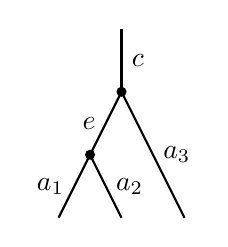
\begin{tikzpicture}[scale=0.8]
    % Left-associated tree: ((a1 ⊗ a2) ⊗ a3) → c
    \draw[thick] (0,0) -- (0.5,1) node[midway, left] {$a_1$};
    \draw[thick] (1,0) -- (0.5,1) node[midway, right] {$a_2$};
    \draw[thick] (0.5,1) -- (1,2) node[midway, left] {$e$};
    \draw[thick] (2,0) -- (1,2) node[midway, right] {$a_3$};
    \draw[thick] (1,2) -- (1,3) node[midway, right] {$c$};
    \filldraw (0.5,1) circle (2pt);
    \filldraw (1,2) circle (2pt);
\end{tikzpicture}
\end{center}
The intermediate channel $e$ ranges over all simple objects with $N_{a_1 a_2}^e \geq 1$ and $N_{e a_3}^c \geq 1$.
\end{example}

\subsection{Fusion Trees as Basis Vectors}

\begin{proposition}[Fusion tree basis]\label{prop:fusion-tree-basis}
The morphism space $\Mor(a_1 \otimes \cdots \otimes a_n, c)$ has a basis indexed by fusion trees with leaves $a_1, \ldots, a_n$ and root $c$. Specifically, for a fixed tree topology $T$ (e.g., left-associated), the basis vectors are indexed by:
\begin{enumerate}
    \item All valid assignments of intermediate channel labels to internal edges.
    \item All valid assignments of multiplicity indices to vertices.
\end{enumerate}
The dimension is
\begin{equation}
    \dim \Mor(a_1 \otimes \cdots \otimes a_n, c) = \sum_{\text{intermediate channels}} \prod_{\text{vertices } v} N_{x_v y_v}^{z_v}
\end{equation}
where the sum runs over all valid channel assignments and the product over all trivalent vertices.
\end{proposition}

\begin{example}[Dimension of $\Mor(a \otimes b \otimes c, d)$]
Using left-association:
\begin{equation}
    \dim \Mor(a \otimes b \otimes c, d) = \sum_{e \in \mathrm{Irr}(\mathcal{C})} N_{ab}^e \, N_{ec}^d.
\end{equation}
This equals $\sum_f N_{bc}^f N_{af}^d$ (right-association) by associativity of the Grothendieck ring.
\end{example}

\subsection{Change of Basis: F-Moves}

\begin{definition}[F-move as basis change]\label{def:f-move-basis}
The \emph{F-move} relates fusion tree bases corresponding to different association orders. For four anyons $a, b, c, d$, the F-symbol $(F_{abc}^d)_{e}^{f}$ (suppressing multiplicity indices) gives the overlap between:
\begin{itemize}
    \item Left-associated basis: $\ket{((a \otimes b) \otimes c) \to d; e}$ with intermediate channel $e$ in $(a \otimes b)$.
    \item Right-associated basis: $\ket{(a \otimes (b \otimes c)) \to d; f}$ with intermediate channel $f$ in $(b \otimes c)$.
\end{itemize}
The change of basis is:
\begin{equation}\label{eq:f-move-cob}
    \ket{(ab)c \to d; e} = \sum_{f} (F_{abc}^d)_{e}^{f} \ket{a(bc) \to d; f}.
\end{equation}
\end{definition}

\begin{remark}[Pentagon as consistency]
The pentagon equation (Definition~\ref{def:pentagon}) ensures that any sequence of F-moves relating two tree topologies yields the same result, regardless of the path taken through intermediate topologies. This is the defining coherence condition for monoidal categories.
\end{remark}

\subsection{Basis Independence}

\begin{convention}[Basis-independent formulations]\label{conv:basis-independence}
Physical quantities and categorical definitions should not depend on:
\begin{enumerate}
    \item The choice of tree topology (left-associated, right-associated, or other).
    \item The choice of multiplicity basis vectors $f_{ab \to c}^{(\mu)}$.
    \item Overall phase conventions for basis morphisms.
\end{enumerate}
Fusion tree bases are a \emph{computational tool}, not part of the categorical structure.
\end{convention}

\begin{remark}[When bases are necessary]
Explicit bases are required for:
\begin{itemize}
    \item Numerical computation of matrix elements (Section~\ref{sec:matrix-elements-2local}).
    \item Defining Hamiltonians in terms of F-symbols.
    \item Interface with TensorCategories.jl and similar software.
\end{itemize}
In such cases, one must verify that final results are basis-independent, or explicitly state which conventions are used.
\end{remark}

\begin{citationblock}
Kitaev, \emph{Anyons in an exactly solved model and beyond}, Ann.~Phys.~321 (2006), Appendix E \cite{Kitaev2006} \unverified
\end{citationblock}
